\chapter{Implementation}
\label{chap:implementation}

\section{Wumpus Platform Robot}
\label{sec:wumpus_platform}
The GolfBot's development started with the Wumpus platform, a pre-existing robot that provided a solid mechanical and electrical base. This section details the initial specifications of the platform, its condition as received, and the critical modifications and improvements that were made.

\subsection{Initial Design and Specifications}
\label{ssec:initial_design}
The Wumpus robot, developed at Maynooth University, is a differential-drive robot. In its original configuration, it was controlled by a Raspberry Pi 4 running ROS 2. The power system was built around a 36V battery, which supplied two VESC motor controllers for the brushless \gls{DC} motors. The platform also included three DC-DC converters: two specifically for the VESC controllers, and a third to step the voltage down to 12V and 5V for the main controller and other peripheral electronics.

\subsection{Base Platform Condition}
\label{ssec:base_condition}
Upon initial inspection, the platform had two key issues that needed to be addressed. First, one of the VESC controllers had a recurring power-up problem. To ensure reliable operation, I installed a dedicated kill switch to control its power flow directly (shown in Figure \ref{fig:appendix_killswitch} in the Appendix). Second, the motor settings were configured for high-speed performance (minimum 900 ERPM), which made the robot uncontrollable at the low speeds required for divot inspection and repair. Using the VESC tool, an open-source configuration software, I lowered the minimum motor speed to 100 ERPM (see Figure \ref{fig:appendix_vesc_tool} in the Appendix). This adjustment was crucial for enabling the precise, low-speed maneuvers needed for the project.

\subsection{Modifications and Improvements} ter J4012, which features a powerful NVIDIA Jetson Orin 16GB module suitable for edge AI computing. I then integrated the following key hardware components:
\begin{itemize}
    \item An Intel RealSense D435i stereo camera for visual and depth data.
    \item An Ardusimple SimpleRTK2B RTK GPS module for high-accuracy localization.
    \item An Arduino Uno microcontroller to manage the dispenser motor and IMU.
    \item A BNO055 IMU sensor for orientation tracking.
    \item An A4988 stepper motor driver and a NEMA 17 stepper motor to actuate the dispenser.
    \item A custom-designed and 3D-printed auger dispenser for the sand-seed mixture.
\end{itemize}
These enhancements fundamentally transformed the general-purpose Wumpus platform into the specialized GolfBot.

\section{Computer Vision System}
\subsection{Introduction/Purpose}
\label{ssec:cv_intro}
The \gls{CV} system is a critical component of the GolfBot, serving as its primary perception system for identifying targets for repair. Its main purpose is to process a live video feed from the onboard camera and use a custom-trained deep learning model to detect and segment divots in real-time.

By leveraging both color (\gls{RGB}) and depth data from the Intel RealSense camera, the system is designed to provide the necessary information for the robot's navigation and control modules to accurately approach and service a detected divot. This section details the entire implementation of the CV system, covering the creation of the dataset, the model training process, the specific hardware and software used, and its final integration into the ROS 2 framework.

\subsection{Data Set Collection and Preprocessing}
\label{ssec:cv_dataset}
The foundation of any effective computer vision model is a high-quality, relevant dataset. The entire workflow, from data collection and annotation to model training and deployment, is illustrated in Figure \ref{fig:cv_workflow}.

\begin{figure}[h!]
    \centering
    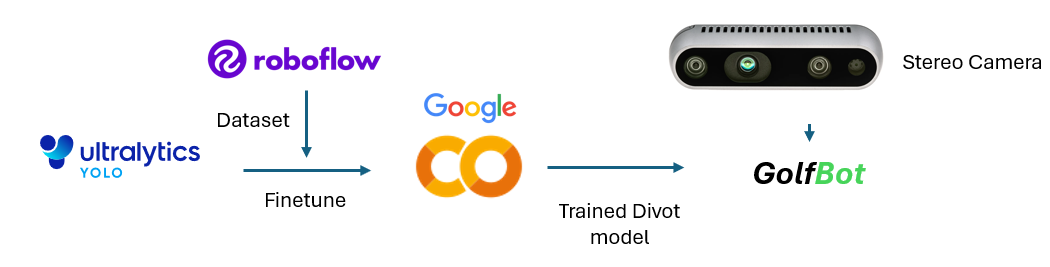
\includegraphics[width=\linewidth]{figures/datasetworkflow.png}
    \caption{The end-to-end computer vision workflow, from data acquisition to a trained model ready for deployment on the GolfBot.}
    \label{fig:cv_workflow}
\end{figure}

\textbf{Data Collection.}
The initial dataset was created by capturing images at a local golf course to ensure the data was representative of real-world conditions. Using a Nikon D5200 DSLR camera, I collected over 1,000 high-resolution images (2992x2000 pixels at 300dpi). These images captured divots in various states, lighting conditions, and turf textures. \textbf{Example images for both the \texttt{divot} and \texttt{fixed\_divots} classes are provided in Appendix \ref{chap:appendix_a} (Figures \ref{fig:appendix_divot_sample} and \ref{fig:appendix_fixed_divot_sample}).}

\textbf{Annotation.}
The collected images were uploaded to the Roboflow online data management platform for annotation. I used Roboflow's "smart polygon" feature to precisely outline the boundaries of each divot, which is essential for instance segmentation. Each annotation was categorized into one of two classes:
\begin{itemize}
    \item \textbf{divot:} An un-repaired patch of displaced turf.
    \item \textbf{fixed\_divot:} A divot that has been filled with a sand-seed mixture.
\end{itemize}
After cleaning and annotating, the dataset consisted of 766 images containing \texttt{divot} instances and 533 images with \texttt{fixed\_divot} instances. This dataset was then split into training (70\%), validation (20\%), and testing (10\%) sets, resulting in 931, 277, and 174 images in each set, respectively.

\textbf{Preprocessing and Augmentation.}
To prepare the images for the model and to increase the dataset's robustness, several steps were applied in Roboflow. First, all images were resized to 640x640 pixels to match the model's expected input dimensions. A contrast-boosting histogram equalization was also applied to normalize the images against varying lighting.

Next, a series of data augmentation techniques were applied to synthetically increase the size and variability of the training set. These included:
\begin{itemize}
    \item \textbf{Crop:} Random cropping up to 20\% to make the model more resilient to objects being partially out of frame.
    \item \textbf{Rotation:} Random rotation of +/- 15 degrees to simulate variations in camera angle.
    \item \textbf{Shear:} Horizontal and vertical shearing of +/- 10\% to account for different viewing perspectives.
    \item \textbf{Exposure:} Random adjustments to image brightness (-10\% to +10\%) to simulate different lighting conditions.
\end{itemize}
These augmentation steps tripled the size of the training dataset, resulting in a final count of 3,244 images for training the model.

\subsection{Model Training}
\label{ssec:cv_training}
The model was trained using the Ultralytics framework, the official maintainer of the YOLO (You Only Look Once) family of models. The training process was executed on the Google Colab platform, which provides access to powerful cloud-based GPUs/TPUs suitable for deep learning tasks.

The training workflow involved the following key steps:
\begin{enumerate}
    \item \textbf{Environment Setup:} The Ultralytics and Roboflow Python libraries were installed in the Google Colab environment.
    \item \textbf{Dataset Download:} The prepared dataset was downloaded directly from Roboflow into the Colab notebook using the Roboflow API. This ensures a direct and reproducible link between the annotated data and the training script.
    \item \textbf{Training Execution:} The training was initiated using the Ultralytics command-line interface. I selected the \textbf{YOLOv11s-seg} model, a small, fast instance segmentation model ideal for edge computing applications like the GolfBot. The model was trained for \textbf{150 epochs} with a \textbf{batch size of 50}.
\end{enumerate}
Upon completion of the training, the resulting model weights file (`best.pt`) was downloaded. This file, which contains the learned parameters of the trained model, was then integrated into the divot detection Python script running on the GolfBot. The quantitative performance of this model is evaluated in Chapter \ref{chap:validation}.

\subsection{Hardware}
\label{ssec:cv_hardware}
The primary sensor for the computer vision system is the Intel RealSense D435i stereo camera, shown in Figure \ref{fig:realsense_camera}. This model was specifically chosen for its dual capabilities, which are central to the project's design.

It provides a high-resolution color (RGB) stream, which serves as the input for the YOLOv11-seg object detection model. In parallel, it features a pair of infrared (IR) stereo sensors. These sensors capture the scene from two slightly different perspectives, allowing the camera's internal vision processor to calculate a dense depth map based on stereo disparity. This depth data is crucial for estimating the real-world size and location of detected divots. The camera connects directly to a USB 3.0 port on the Jetson controller, ensuring sufficient bandwidth for real-time image and depth data streaming.

\begin{figure}[h!]
    \centering
    % Put your realsense camera image here
    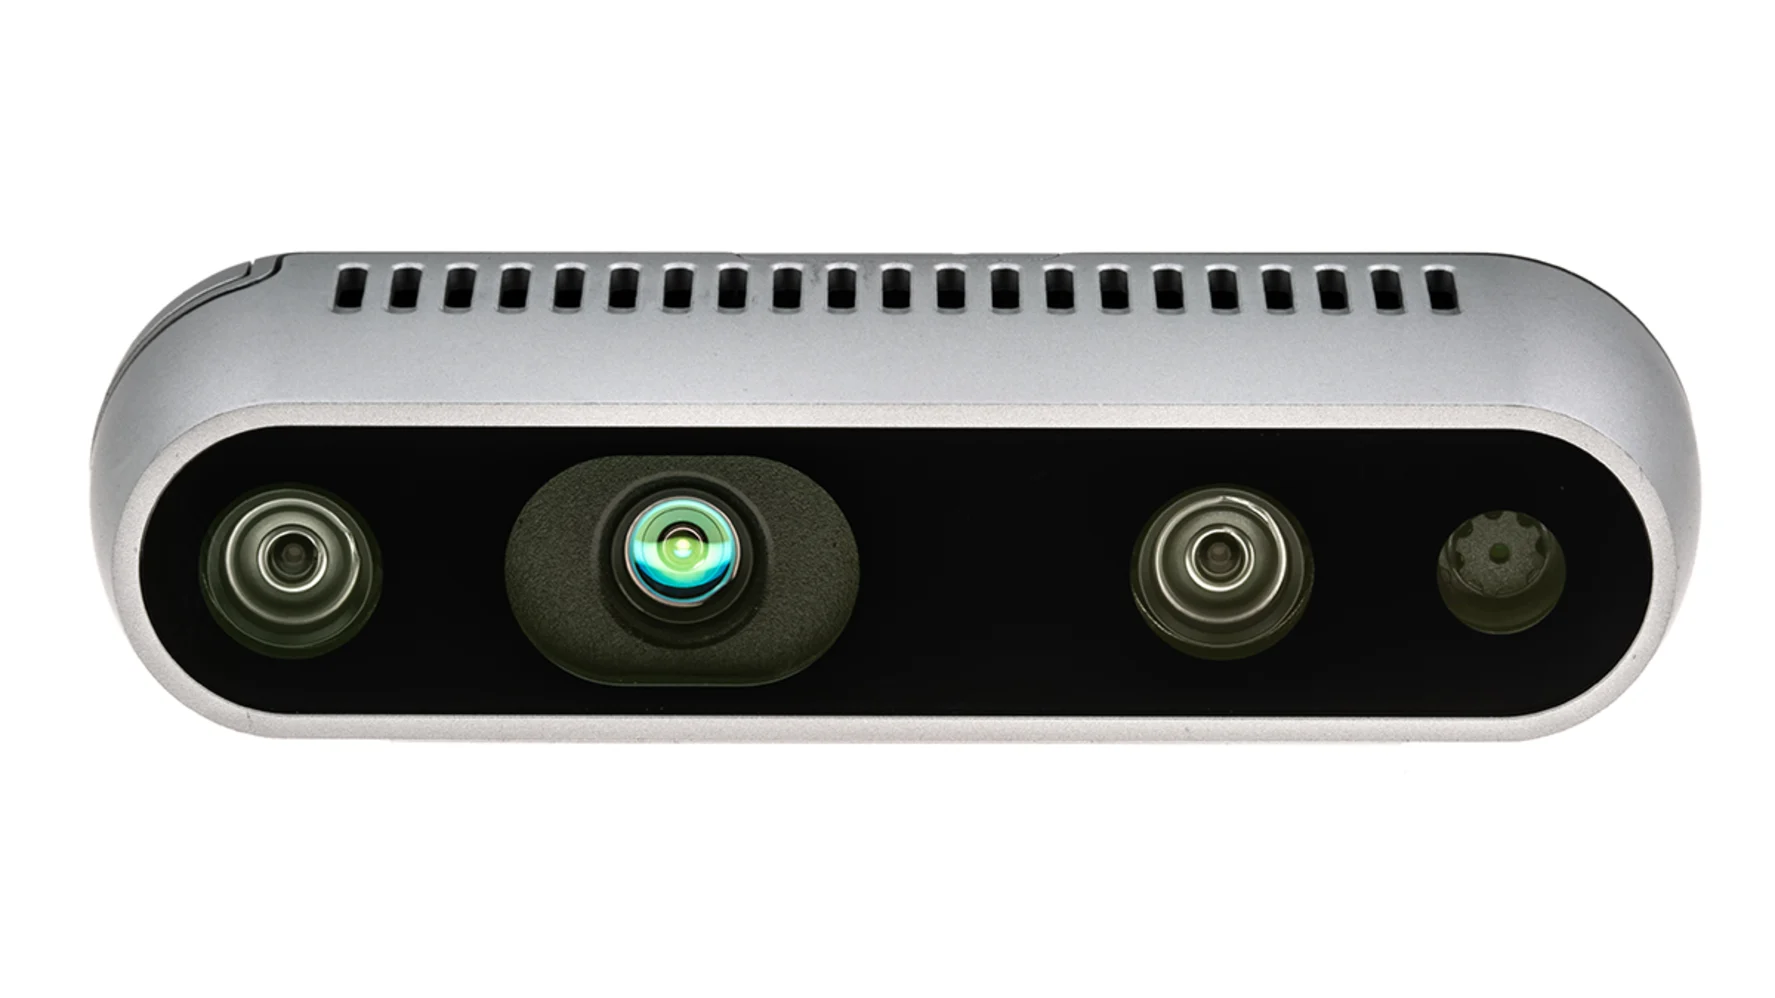
\includegraphics[width=0.6\linewidth]{figures/camera.png}
    \caption{The Intel RealSense D435i camera used for the computer vision system.}
    \label{fig:realsense_camera}
\end{figure}

\subsection{Software}
\label{ssec:cv_software}
The computer vision system is implemented in Python and relies on a curated set of powerful, open-source libraries to create a robust data pipeline. These libraries handle everything from low-level camera interfacing to high-level model inference and data visualization. Key code listings illustrating the use of these libraries can be found in Appendix \ref{chap:appendix_a}, Section \ref{sec:appendix_code}

\begin{description}
    \item[Ultralytics YOLO] This is the core library for the AI-based detection. As seen in the \texttt{divot\_detector\_node}, this package is used to load the custom-trained \texttt{.pt} model file and run inference on the incoming video stream. It provides a high-level, efficient interface to the state-of-the-art YOLOv11 model architecture.

    \item[Supervision] The \texttt{supervision} library is used extensively for post-processing the output from the YOLO model. Its utilities simplify common computer vision tasks. In this project, it is used to convert the raw model output into an easily accessible detections object, and to annotate the video frames with segmentation masks, bounding boxes, and labels for visualization.

    \item[PyRealSense2] This is the official Python wrapper for the Intel RealSense SDK. It is the fundamental library used in the \texttt{camera\_node} to directly interface with the D435i camera. It handles the configuration of the camera streams (color and depth), frame alignment, and retrieval of the image data.

    \item[OpenCV] The Open Source Computer Vision Library (OpenCV) is a foundational component used throughout the pipeline. It is primarily used for image data manipulation. For instance, it is used by the \texttt{CvBridge} library to handle image format conversions and by the \texttt{divot\_detector\_node} to draw diagnostic visualizations, such as circles and text, onto the final annotated image.

    \item[CvBridge] This is a critical ROS 2 utility library that acts as the "bridge" between ROS \texttt{sensor\_msgs/Image} messages and the OpenCV image format. It is used in both the \texttt{camera\_node} (to convert captured frames into ROS messages) and the \texttt{divot\_detector\_node} (to convert received ROS messages back into a format that OpenCV and the YOLO model can process).

    \item[NumPy] As the fundamental package for scientific computing with Python, NumPy is used implicitly by most other libraries. It is explicitly used in the \texttt{divot\_detector\_node} for all numerical operations, such as calculating the center coordinates of a segmentation mask from pixel arrays and performing the geometric calculations for area and distance estimation.
\end{description}
Together, these libraries form a complete and efficient pipeline, enabling the GolfBot to process visual information from the physical world into actionable data within the ROS 2 ecosystem.

\subsection{Implementation in ROS}
\label{ssec:cv_ros_implementation}
With a trained model ready, the final implementation step was to integrate it into a ROS 2 node that could run on the GolfBot. The \texttt{/divot\_detector} node was created for this purpose. Its operational logic follows a clear, multi-stage pipeline for each incoming image, as illustrated in Figure \ref{fig:cv_processing_pipeline}.

\begin{figure}[h!]
    \centering
    \includegraphics[width=0.9\linewidth]{figures/cv_pipeline_grid.png}
    \caption{The real-time computer vision processing pipeline. The top row shows an original captured image being processed to create a segmentation mask. The bottom row illustrates the subsequent classification and depth analysis steps.}
    \label{fig:cv_processing_pipeline}
\end{figure}

The node subscribes to the \texttt{/camera/color/image\_raw} topic. For each image received, it executes the following sequence:

\begin{enumerate}
    \item \textbf{Instance Segmentation:} The raw image is first passed to the YOLOv11-seg model. The model identifies and generates a precise pixel-level segmentation mask for any object it recognizes as a divot or a fixed divot.

    \item \textbf{Divot Classification:} For each segmented instance, the model provides a classification (either \texttt{divot} or \texttt{fixed\_divot}) along with a confidence score (e.g., \texttt{divot 0.92}). This allows the system to distinguish between areas that need repair and those that have already been serviced.

    \item \textbf{Depth Estimation:} Once a divot is positively identified and segmented, its pixel mask is used to query the corresponding depth data from the RealSense camera's aligned depth stream. While calculating the full volume was deferred as future work, this step confirms that the necessary 3D data can be extracted for a specific, non-rectangular target.
\end{enumerate}

After this pipeline is complete, the results — including the annotated image with segmentation masks, structured details about the detections, and performance metrics — are published to their respective ROS 2 topics for use by the GUI and navigation systems.

\section{Navigation System}
\subsection{Introduction/Purpose}
\subsection{Hardware Used}
\subsection{Software Implementation}

\section{Mechanical Dispenser}
\subsection{Introduction/Purpose}
\subsection{Hardware Design and 3D-Printed Components}
Here I can specify the output rate of the dispenser and the volume of the sand-seed mixture that is dispensed.
\subsection{Software Integration in ROS}

\section{Graphical User Interface (GUI)}
\subsection{Introduction/Purpose}
\subsection{Software and Framework}
\subsection{Functions, Features, and Control}

% %Section: Computer Vision System
% Introduction/Purpose: A brief one-paragraph reminder of the goal: to detect divots from a camera feed.
% Data Set Collection and Preprocessing: This is pure implementation.
% How did you collect the 689 images? (e.g., "Images were collected over several days at the Maynooth University campus golf facility under varying lighting conditions...")
% How did you use Roboflow? Describe the process of uploading, annotating the two classes (divot and fixed_divot), and exporting the dataset.
% What specific data augmentations did you apply? Mention the exact transformations like rotation (e.g., +/- 15 degrees), brightness changes (e.g., +/- 25), etc., that expanded the dataset to 1,653 images.
% Model Training:
% Describe the training process on Google Colab. Mention the key parameters: 100 epochs, the specific YOLOv11-seg model used, and the fact that you used TPUs.
% Hardware: You described the camera in the Design chapter. Here, you describe its setup.
% "The Intel RealSense D435i was configured using the pyrealsense2 library to stream RGB video at a resolution of 1280x720 and 30 frames per second."
% Software: List the key libraries you used.
% pyrealsense2 for camera interfacing, OpenCV for image manipulation, and the ultralytics Python package for running the YOLO model inference.
% Implementation in ROS: This is critical.
% Describe your ROS 2 node (divot_detection_intel.py).
% Specify the topics it subscribes to (/camera/color/image_raw) and publishes to (/camera/divot_detection/image_raw, /camera/divot_detection/details).
% Mention the message types (sensor_msgs/Image). You could even include a small, simplified code snippet of your main processing loop.

% Section: Navigation System
% Introduction/Purpose: Reminder of the goal: achieve centimeter-level navigation.
% Hardware Used: Again, focus on the configuration.
% "The ArduSimple simpleRTK2B rover module was configured to output NMEA sentences at 10 Hz over USB."
% "The BNO055 IMU was interfaced with the Arduino, which was programmed to read the fused orientation data and send it over its serial port."
% Software Implementation:
% Explain how you used the ublox_gps_node ROS 2 package to read the data from the ArduSimple module and publish it to the /fix topic.
% Describe your stepper_imu_node.py, explaining how it reads the serial data from the Arduino and publishes it as a sensor_msgs/Imu message on the /imu/data topic.
% This is the perfect place to describe the simple "lawnmower" search algorithm you implemented for autonomous coverage.


% Section: Mechanical Dispenser
% Introduction/Purpose: Reminder of the goal: dispense a controlled amount of sand/seed mix.
% Hardware Design and 3D-Printed Components: You are exactly right with your idea for this section.
% In the Design chapter, you described what it looks like and where it is.
% Here, in Implementation, you describe how it performs. "The auger was designed in Fusion 360 and 3D-printed using PLA. Through a series of tests, it was calibrated to determine its output rate. Running the NEMA 17 stepper motor for X seconds at Y speed dispenses an average of Z grams of the sand-seed mixture. The hopper has a total volume of..."
% Software Integration in ROS:
% Explain the simple serial protocol you created (e.g., sending the character 'R' to run the motor and 'S' to stop it).
% Describe the part of your stepper_imu_node.py that sends these characters to the Arduino's serial port when a joystick button is pressed.
% You could include the simple Arduino code snippet (if (Serial.available() > 0) ...) that listens for these commands and drives the A4988 stepper driver.
% Section: Graphical User Interface (GUI)
% Introduction/Purpose: To provide teleoperation and system monitoring.
% Software and Framework: Describe what you used to build it. (e.g., "The GUI was developed as an RQT plugin using Python and the PyQt5 framework.")
% Functions, Features, and Control:
% Detail what the user can see and do. Show a screenshot.
% "The GUI displays the live camera feed, the annotated divot detection feed, the current RTK GPS status (Fixed, Float, None), and provides buttons for manual control, starting the autonomous mode, and triggering the dispenser."
